\documentclass[11pt]{article}

\usepackage[margin=1.05in]{geometry}
\usepackage{amsmath,amssymb,amsthm}
\usepackage{mathtools}
\usepackage{graphicx}
\usepackage{booktabs}
\usepackage{array}
\usepackage{microtype}
\usepackage{xcolor}
\usepackage[shortlabels]{enumitem}
\usepackage[colorlinks=true,linkcolor=blue!45!black,citecolor=blue!45!black,urlcolor=blue!45!black]{hyperref}
\hypersetup{pdftitle={Endpoint crossings in the persistent random walk: uniform Bessel bounds and boundary effects},pdfauthor={Arjun Pemmasani}}

% ---------- theorem environments ----------
\newtheorem{theorem}{Theorem}[section]
\newtheorem{lemma}[theorem]{Lemma}
\newtheorem{proposition}[theorem]{Proposition}
\newtheorem{corollary}[theorem]{Corollary}
\theoremstyle{definition}
\newtheorem{definition}[theorem]{Definition}
\newtheorem{example}[theorem]{Example}
\theoremstyle{remark}
\newtheorem{remark}[theorem]{Remark}

% ---------- notation macros ----------
\newcommand{\Z}{\mathbb{Z}}
\newcommand{\E}{\mathbb{E}}
\newcommand{\Prob}{\mathbb{P}}
\newcommand{\Var}{\operatorname{Var}}
\newcommand{\Cov}{\operatorname{Cov}}
\newcommand{\chg}{\operatorname{chg}}
\newcommand{\rep}{\operatorname{rep}}

\title{Endpoint crossings in the persistent random walk:\\
uniform Bessel bounds and boundary effects}
\author{Arjun Pemmasani}
\date{September 22, 2026}
\begin{document}
\maketitle

\begin{abstract}
For a symmetric persistent random walk, we bound the relative error of a
Bessel approximation to the ratio of each interior bin probability to an
endpoint probability. If there are $N$ steps and the switching odds are
$u=(1-p)/p$, the relative error is at most $Nu^2/2+u$, whatever the bin. From
this we get an expansion of the crossing point, with explicit constants and
a $1/\log$ correction, that holds for all bins at a distance from the edge
tending to infinity. For a bin at a fixed distance from the edge, the
crossing comes instead from a finite Laguerre polynomial, and the next term
turns out to be the same for all such bins. We also show that the two
regimes match. We then prove the same kind of bound for periodic spin
boundaries. The periodic and free central crossings differ in odds by
$(\log 2)/N$ to leading order. In both cases the ratio near the center looks
like $\exp(t-2y^2)$, which tells us how many bins sit above the endpoints.
The exact law, the normal limit and the Bessel scaling were known before,
and so was the question of when the middle and the endpoints are equal. Our
results are about how big the discrete error is when $p$ and the bin change
with $N$.
\end{abstract}

\section{Introduction}\label{sec:intro}

Problem 131 of Kagey's Open Problem Collection~\cite{kagey131} asks about
a Galton board where the ball tends to keep going the same way. The first
step is equally likely to be left or right, and after that each step
repeats the one before it with probability $p$. In particular, it asks when
the middle bin and the endpoints have equal probability. We study that
comparison for every interior bin, including bins approaching an edge,
and compare free and periodic spin boundaries.

\paragraph{Model and conventions.}
Let $P_N(k)$ denote the probability of exactly $k$ right steps in $N$
steps, with $P_0(0)=1$. Write $q=1-p$, $\rho=2p-1$, and $u=q/p$ when
$p>0$. Thus $P_N(0)=P_N(N)=p^{N-1}/2$ for $N\ge1$.
Kagey's row $n$ corresponds to $N=n-1$. For $p=\alpha/(\alpha+\beta)$,
his numerator tables are
\[
 n_N(k)=2(\alpha+\beta)^{N-1}P_N(k)\quad(N\ge1),\qquad n_0(0)=1.
\]
These are the numerators as Kagey tabulates them, not reduced fractions.

\paragraph{Results and organization.}
Our main estimate, Theorem~\ref{thm:allbin-bessel}, bounds the relative
error of a Bessel majorant independently of the bin. Its consequences
are a crossing expansion uniform over every growing edge distance
(Theorem~\ref{thm:allbin-expansion}), a fixed-edge Laguerre law and its
matching limit (Theorems~\ref{thm:edge-laguerre} and~\ref{thm:edge-matching}),
and the periodic/free boundary shift and spatial critical window in
Section~\ref{sec:periodicwindow}. We first give short proofs of the exact
law, the lattice-path interpretations of Kagey's two numerator tables,
and the variance and normal limit. Section~\ref{sec:middle} proves that
the central crossing is unique and strictly increasing in $N$. The
all-bin theorem also gives the central expansion, but we treat the center
separately since the inversion is simplest there.

\paragraph{Prior work.}
The correlated random walk goes back to Goldstein~\cite{goldstein1951}
and Gillis~\cite{gillis1955}. Renshaw and Henderson~\cite{renshaw1981}
study the same symmetric model, motivated by a Galton machine, and give the
exact law from run counts, the generating function, the normal limit, and
the upturn at the endpoints. Their Section~4 also gives a Bessel limit at a
fixed persistence scale, followed by a limit as that scale grows. Since the
two limits are taken one after the other, they do not give an error bound at
finite $N$ when the scale grows like $\log N$, which is where the crossing
happens. The run count used below is classical~\cite{waldwolfowitz1940}.
Dekking and Kong~\cite{dekkingkong2011} give the Markov-binomial law, the
variance, and a classification of the local modes. Their Proposition~4.3
proves interior log-concavity for an arbitrary initial distribution and
$0<a,b<1$, and our model is the case $a=b=1-p$ with a symmetric initial law.
We prove the ordering we need directly from the coefficients instead. The
OEIS entries already record both tables~\cite{oeisA035002,oeisA348595}, and
our bijections explain the connections Kagey points out.

Herrmann and Vallois~\cite{herrmann2010} give the telegraph limit with
its Bessel density. Antal, Droz and R\'acz~\cite{antal2004} treat the
magnetization distribution at fixed scale under several boundary conditions,
and Dantchev and Rudnick~\cite{dantchev2022} give exact free and periodic
coefficients. Stepanyan et al.~\cite[Section~III.B]{stepanyan2024} study the
periodic endpoint--adjacent and endpoint--center crossings directly and give a
finite-size approximation to the latter~\cite[Eq.~(16)]{stepanyan2024}. So we
did not come up with the crossing question. Our part is bounding the discrete
error when $Nu=O(\log N)$ (and near the edges), solving for the crossing from
that bound, and finding the window of bins above the endpoints. The Markov-binomial estimates
in~\cite{cekanavicius2001,cekanavicius2001ld} assume ranges of the transition
probabilities that exclude the symmetric limit $p\to1$.

\section{The exact distribution}\label{sec:exact}

A run of the experiment with $N\ge1$ bounces is a word $w\in\{L,R\}^N$. Let $\chg(w)$ be the number of
indices $i<N$ with $w_i\ne w_{i+1}$ and $\rep(w)=N-1-\chg(w)$. By the definition of the model,
\begin{equation}\label{eq:wordprob}
\Prob(w)=\tfrac12\,p^{\rep(w)}q^{\chg(w)} .
\end{equation}

\begin{theorem}[bin probabilities]\label{thm:pmf}
Let $N\ge1$. Then $P_N(0)=P_N(N)=\tfrac12p^{N-1}$, and for $1\le k\le N-1$
\[
P_N(k)=\frac12\sum_{j=1}^{N-1}W(N,k,j)\,p^{N-1-j}q^{\,j},
\]
where, writing $a=k$ and $b=N-k$,
\[
W(N,k,2i-1)=2\binom{a-1}{i-1}\binom{b-1}{i-1},\qquad
W(N,k,2i)=\binom{a-1}{i}\binom{b-1}{i-1}+\binom{a-1}{i-1}\binom{b-1}{i}
\]
is the number of words with $a$ letters $R$, $b$ letters $L$ and exactly $j$ direction changes.
\end{theorem}

\begin{proof}
By \eqref{eq:wordprob} it suffices to count words. A word with $j$ changes consists of $j+1$ maximal
runs, alternately of $R$'s and of $L$'s. If $k\in\{0,N\}$ there is one word and it has no change.
Let $a,b\ge1$. If $j+1=2i$ there are $i$ runs of each letter and the first letter is free. The run
lengths form a composition of $a$ into $i$ parts and a composition of $b$ into $i$ parts, and there
are $\binom{a-1}{i-1}\binom{b-1}{i-1}$ such pairs. If $j+1=2i+1$ the word starts and ends with the
same letter. Starting with $R$ gives $i+1$ runs of $R$ and $i$ runs of $L$, so
$\binom{a-1}{i}\binom{b-1}{i-1}$ words, and starting with $L$ gives the other summand.
\end{proof}

For instance $P_2=(\tfrac p2,\,q,\,\tfrac p2)$, $P_3(1)=P_3(2)=\tfrac12(1-p^2)$ and
$P_4(2)=(1-p)(1-p+p^2)$.

Note that the only way to end in bin $0$ is the word $L\cdots L$, which never switches. Every
other bin needs at least one switch. So when $p$ is close to $1$ the endpoints win, and the
question in Section~\ref{sec:middle} is how close $p$ has to be.

\begin{proposition}[recurrence and generating function]\label{prop:gf}
Let $R_N(k)$ and $L_N(k)$ be the probabilities of being in bin $k$ after $N$ bounces with last bounce
$R$, respectively $L$. Then $R_1(1)=L_1(0)=\tfrac12$ and
\begin{equation}\label{eq:dp}
R_N(k)=p\,R_{N-1}(k-1)+q\,L_{N-1}(k-1),\qquad L_N(k)=p\,L_{N-1}(k)+q\,R_{N-1}(k).
\end{equation}
Consequently
\begin{equation}\label{eq:gf}
\sum_{N\ge0}\sum_{k=0}^{N}P_N(k)\,x^kt^N=\frac{1-(p-\tfrac12)(1+x)\,t}{1-p(1+x)\,t+(2p-1)\,x\,t^2},
\end{equation}
and for all $N\ge2$ and all $k$ (with $P_M(k)=0$ outside $0\le k\le M$)
\begin{equation}\label{eq:rec}
P_N(k)=p\bigl(P_{N-1}(k)+P_{N-1}(k-1)\bigr)-(2p-1)\,P_{N-2}(k-1).
\end{equation}
\end{proposition}

\begin{proof}
The recursion \eqref{eq:dp} follows by conditioning on the last two bounces. Put $F_R=\sum R_N(k)x^kt^N$ and
$F_L=\sum L_N(k)x^kt^N$. Then \eqref{eq:dp} and the initial values give
$F_R=xt\bigl(\tfrac12+pF_R+qF_L\bigr)$ and $F_L=t\bigl(\tfrac12+pF_L+qF_R\bigr)$. The determinant of
this linear system is $(1-pxt)(1-pt)-q^2xt^2=1-p(1+x)t+(p^2-q^2)xt^2$, and $p^2-q^2=2p-1$. Cramer's
rule gives $F_R=\tfrac12xt\,(1-\rho t)/\Delta$ and $F_L=\tfrac12t\,(1-\rho xt)/\Delta$ with $\Delta$
the determinant, and $1+F_R+F_L$ simplifies to \eqref{eq:gf}. Multiplying \eqref{eq:gf} by $\Delta$
and reading off the coefficient of $x^kt^N$ for $N\ge2$ gives \eqref{eq:rec}.
\end{proof}

At $p=\tfrac12$ the last term of \eqref{eq:rec} vanishes and \eqref{eq:rec} is Pascal's rule with
weights $\tfrac12$. In terms of numerators, \eqref{eq:rec} reads
$n_N(k)=\alpha\bigl(n_{N-1}(k)+n_{N-1}(k-1)\bigr)-(\alpha^2-\beta^2)\,n_{N-2}(k-1)$ for $N\ge3$.

\section{The numerator tables and lattice paths}\label{sec:tables}

\begin{proposition}\label{prop:num}
Let $p=\alpha/(\alpha+\beta)$ with integers $\alpha,\beta\ge0$, not both zero. For $N\ge1$,
\[
n_N(k)=\sum_{w}\alpha^{\rep(w)}\beta^{\chg(w)},
\]
the sum over the words with $k$ letters $R$ and $N-k$ letters $L$. In particular the numerators are
integers, and
\[
\sum_{a,b\ge0}n_{a+b}(a)\,x^ay^b=
\frac{1-(\alpha-1)(x+y)+(\alpha-\beta)(\alpha+\beta-2)\,xy}{1-\alpha(x+y)+(\alpha^2-\beta^2)\,xy}.
\]
\end{proposition}

\begin{proof}
Multiply \eqref{eq:wordprob} by $2(\alpha+\beta)^{N-1}$. For the generating function, let $F_R$ and
$F_L$ be the sums of the weighted words ending in $R$ and in $L$. Then $F_R=x(1+\alpha F_R+\beta F_L)$ and
$F_L=y(1+\alpha F_L+\beta F_R)$, and solving as in Proposition~\ref{prop:gf} gives the stated
value of $1+F_R+F_L$.
\end{proof}

For $(\alpha,\beta)=(2,1)$ the generating function is $(1-x)(1-y)/(1-2x-2y+3xy)$, and for
$(\alpha,\beta)=(1,2)$ it is $(1-xy)/(1-x-y-3xy)$. These are the generating functions recorded in
A035002 (by Kruchinin and by Somos) and in A348595 (by Mathar) \cite{oeisA035002,oeisA348595}, which already identifies the
tables. We prove the identifications directly from the definitions of the two sequences, which
shows where the weights $2$ come from.

\begin{theorem}[$p=\tfrac23$ and rook paths]\label{thm:rook}
Let $T(a,b)$ be the number of ways to move a rook from $(0,0)$ to $(a,b)$ by moves that increase one
coordinate by a positive amount. Then for $p=\tfrac23$, $n_N(k)=T(k,N-k)$ for all $N\ge0$ and
$0\le k\le N$. In the indexing of A035002, whose array starts at $(1,1)$, this is the entry $(k+1,N-k+1)$, so
Kagey's $p=\tfrac23$ table read by rows is A035002 read by antidiagonals.
\end{theorem}

\begin{proof}
A035002 is defined by the rule that each entry is the sum of all entries to its left and all entries
above it, which is the recursion for $T$ obtained by removing the last rook move (the OEIS entry
records this interpretation). Given a rook path to $(a,b)$ with $a+b=N\ge1$, replace each move of
length $\ell$ to the right by $R^\ell$ and each move of length $\ell$ upward by $L^\ell$. This
gives a word $w$ with $a$ letters $R$ and $b$ letters $L$, together with the set of positions
$i<N$ at which one move ends and the next begins. Such a cut is forced wherever
$w_i\ne w_{i+1}$ and is optional wherever $w_i=w_{i+1}$, and every choice of optional cuts comes from
exactly one rook path. Hence, $T(a,b)=\sum_w2^{\rep(w)}$, which is $n_N(a)$ for
$(\alpha,\beta)=(2,1)$ by Proposition~\ref{prop:num}.
\end{proof}

\begin{theorem}[$p=\tfrac13$ and Mathar's blocked walks]\label{thm:mathar}
Call a lattice point $(x,y)$ \emph{blocked} if $x\equiv y\equiv1$ or $x\equiv y\equiv2\pmod 3$. Let
$M(a,b)$ be the number of walks from $(0,0)$ to $(3a,3b)$ with unit steps right and up that visit no
blocked point. Then for $p=\tfrac13$, $n_N(k)=M(k,N-k)$. The array $M$ is symmetric, and A348595
lists its lower triangle $M(n,k)$, $0\le k\le n$. This is the sense in which that entry is
``related'' to the $p=\tfrac13$ table.
\end{theorem}

\begin{proof}
Reduce coordinates modulo $3$. The allowed residues are $(0,0)$, $(1,0)$, $(2,0)$, $(2,1)$, $(0,1)$,
$(0,2)$, $(1,2)$. We call a point with residue $(0,0)$ a \emph{corner}. Let $X$ be the number of
times the walk steps onto a vertical line $x\equiv0$, and $Y$ the number of times it steps onto a
horizontal line $y\equiv0$. From a corner the walk goes right or up. After a right step it is at
residue $(1,0)$, and up is blocked, so it goes on to $(2,0)$. Call this state $\mathsf A$. From
$\mathsf A$, a right step lands on a corner and increases $X$. An up step leads to $(2,1)$, where up
is blocked, so the walk goes right to $(0,1)$, which increases $X$, and then up to $(0,2)$ since
right is blocked. Call this state $\mathsf B$. By symmetry, an up step from a corner leads to
$\mathsf B$ without changing $X$ or $Y$, and from $\mathsf B$ the walk reaches either a corner or
$\mathsf A$, with $Y$ going up by one either way.

So each visit to $\mathsf A$ gives one letter $R$ (an increase of $X$) and is followed by a corner
or by $\mathsf B$. Each visit to $\mathsf B$ gives one letter $L$ and is followed by a corner or by
$\mathsf A$. A corner leads to $\mathsf A$ or $\mathsf B$ and gives no letter. Hence a walk from the
corner $(0,0)$ to the corner $(3a,3b)$ gives a word $w$ with $a$ letters $R$ and $b$ letters $L$,
where $w_i$ comes from a visit to $\mathsf A$ if it is $R$ and to $\mathsf B$ if it is $L$. Between
$w_i$ and $w_{i+1}$ the walk goes from one of these states to the next. If $w_i=w_{i+1}$ it has to
pass through a corner, so there is one way. If $w_i\ne w_{i+1}$ it can pass through a corner or go
directly, so there are two ways. The start and the end are forced. Hence
$M(a,b)=\sum_w2^{\chg(w)}$, which is $n_N(a)$ for $(\alpha,\beta)=(1,2)$. In Mathar's note
\cite{mathar2022} attached to A348595, the ``squares'' in the name of the sequence are the lattice
points $(x,y)$ themselves, as his recurrences show, so $M$ is his count. Counting the walks directly
also gives the published terms (Section~\ref{sec:verify}).
\end{proof}

Figure~\ref{fig:lattice} shows both bijections for the word $RRLRLL$.

\begin{figure}[t]
\centering
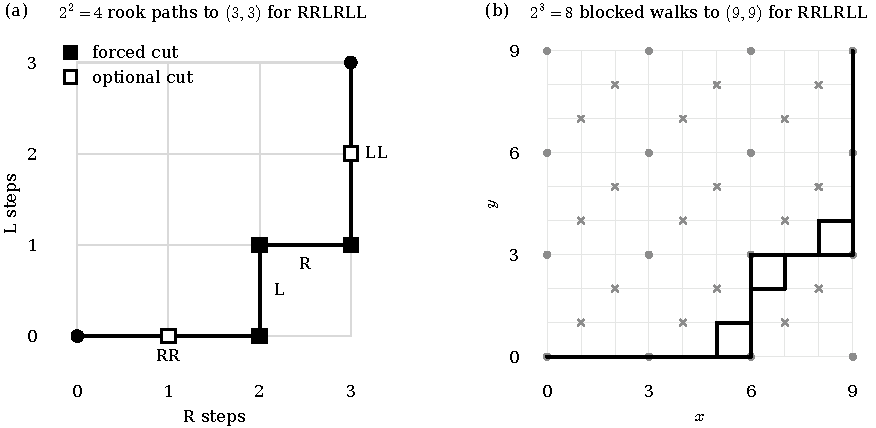
\includegraphics{figures/lattice}
\caption{The two bijections for the word $RRLRLL$. (a) The rook path. A cut
is forced at each of the $3$ direction changes (filled) and optional between
equal letters (hollow), so the word comes from $2^2=4$ rook paths to $(3,3)$.
(b) The union of the $2^3=8$ blocked walks to $(9,9)$ that give the word,
with one detour square for each direction change. Blocked points are marked
$\times$ and corners by dots.}
\label{fig:lattice}
\end{figure}

For general $p=\alpha/(\alpha+\beta)$, Proposition~\ref{prop:num} says that $n_N(k)$ counts monotone
lattice paths from $(0,0)$ to $(k,N-k)$ in which each straight continuation is colored in one of
$\alpha$ ways and each corner in one of $\beta$ ways. This gives the general weighted lattice-path interpretation.

\section{Variance and the normal limit}\label{sec:clt}

Write $e_i=+1$ if the $i$-th bounce is $R$ and $e_i=-1$ otherwise, $X_N=e_1+\dots+e_N$, and
$K_N=(N+X_N)/2$ for the bin index. Then $e_{i+1}=e_is_i$, where $s_1,s_2,\dots$ are independent of
each other and of $e_1$, with $\Prob(s_i=1)=p$ and $\Prob(s_i=-1)=q$, so $\E s_i=\rho$.

\begin{proposition}[mean and variance]\label{prop:var}
$\E K_N=N/2$, and for $p<1$
\[
\Var K_N=\frac14\Bigl(N\,\frac{1+\rho}{1-\rho}-\frac{2\rho\,(1-\rho^N)}{(1-\rho)^2}\Bigr)
=\frac{Np}{4(1-p)}-\frac{(2p-1)\bigl(1-(2p-1)^N\bigr)}{8(1-p)^2}.
\]
For $p=1$, $\Var K_N=N^2/4$.
\end{proposition}

\begin{proof}
Note that $\E e_1=0$ and $e_{i+m}=e_is_i\cdots s_{i+m-1}$, so $\E e_i=0$ and
$\E e_ie_{i+m}=\rho^m$. Hence,
$\Var X_N=N+2\sum_{m=1}^{N-1}(N-m)\rho^m$. Summing the two geometric series gives the first
form, and the second follows from $(1+\rho)/(1-\rho)=p/q$ and $1-\rho=2q$.
\end{proof}

\begin{theorem}[normal limit]\label{thm:clt}
Let $0<p<1$. Then $(K_N-N/2)/\sqrt N$ converges in distribution to the normal law with mean $0$ and
variance $p/(4(1-p))$.
\end{theorem}

\begin{proof}
Let $\varphi_N(\theta)=\E e^{i\theta X_N}$ and let $v_N$ be the column vector with entries
$\E\bigl[e^{i\theta X_N};e_N=+1\bigr]$ and $\E\bigl[e^{i\theta X_N};e_N=-1\bigr]$. By \eqref{eq:dp},
$v_{N+1}=Mv_N$ with
\[
M=\begin{pmatrix}pe^{i\theta}&qe^{i\theta}\\qe^{-i\theta}&pe^{-i\theta}\end{pmatrix},\qquad
\operatorname{tr}M=2p\cos\theta,\quad\det M=p^2-q^2=\rho .
\]
The eigenvalues are $\lambda_\pm(\theta)=p\cos\theta\pm\sqrt{q^2-p^2\sin^2\theta}$, using
$p^2-\rho=q^2$. For $|\sin\theta|<q/p$ they are real and distinct, so
$\varphi_N=c_+\lambda_+^{N-1}+c_-\lambda_-^{N-1}$ for $N\ge1$, with $c_\pm(\theta)$ determined by
$\varphi_1=\cos\theta$ and $\varphi_2=p\cos2\theta+q$, which give
\[
c_+=\frac{\varphi_2-\lambda_-\cos\theta}{\lambda_+-\lambda_-},\qquad c_-=\cos\theta-c_+ .
\]
As $\theta\to0$ we have $\lambda_+\to1$, $\lambda_-\to\rho$, $c_+\to1$, $c_-\to0$, and
\[
\lambda_+(\theta)=p\bigl(1-\tfrac{\theta^2}2\bigr)+q\Bigl(1-\frac{p^2\theta^2}{2q^2}\Bigr)+O(\theta^4)
=1-\frac{p}{2q}\,\theta^2+O(\theta^4).
\]
Fix $s\in\mathbb R$ and put $\theta=s/\sqrt N$. Since $|\rho|<1$, $c_-\lambda_-^{N-1}\to0$, and
$\lambda_+^{N-1}\to\exp\bigl(-\tfrac{p}{2q}s^2\bigr)$. Hence, $\varphi_N(s/\sqrt N)\to
\exp\bigl(-\tfrac{p}{2q}s^2\bigr)$, and by L\'evy's continuity theorem
\cite[Theorem~26.3]{billingsley1995} $X_N/\sqrt N$ converges to the normal law with variance
$p/q$. Finally $K_N-N/2=X_N/2$.
\end{proof}

For $p=1$ the ball is in bin $0$ or bin $N$ with probability $\tfrac12$ each, and for $p=0$ it is
in a middle bin, so there is no normal limit in these two cases.

\begin{remark}[cylinder]\label{rem:cyl}
On a cylinder whose rows have $c$ pegs the local rule is unchanged, so the position is $X_N$ modulo
$2c$ (in half-peg units), and the discrete Fourier coefficients of its law are
$\varphi_N(\pi l/c)$, $0\le l<2c$. The formula $\varphi_N=c_+\lambda_+^{N-1}+c_-\lambda_-^{N-1}$
holds whenever $\lambda_+\neq\lambda_-$. For $0<p<1$ and $\theta\notin\pi\Z$ both eigenvalues have
modulus less than $1$. Real eigenvalues satisfy $|\lambda_\pm|\le p|\cos\theta|+q$, and complex
ones have modulus $\sqrt\rho$. The coefficients at $l=0$ and $l=c$ are $1$ and $(-1)^N$. Hence, on
the cylinder the law approaches the uniform law on the $c$ positions of the correct parity
geometrically fast, and there is no normal shape in the limit.
\end{remark}

\section{When does the middle equal the extremes?}\label{sec:middle}

Let $N\ge2$ and let $m_N=\lfloor N/2\rfloor$ be a middle bin (for odd $N$ the two middle bins have
equal probability by symmetry). Put $u=q/p$. By Theorem~\ref{thm:pmf},
\begin{equation}\label{eq:SN}
\frac{P_N(m_N)}{P_N(0)}=S_N(u):=\sum_{j=1}^{N-1}W(N,m_N,j)\,u^j ,
\end{equation}
a polynomial in $u$ with nonnegative integer coefficients and $W(N,m_N,1)=2$.

We expect $1-p_N$ to be about $(\log N)/N$. Each switch in a word gives a factor of $u$, and a
word that ends in the middle can switch almost anywhere, so adding them up gives roughly
$e^{Nu}/N$. This is $1$ when $Nu\approx\log N$. Theorem~\ref{thm:bessel} proves this with the
correction terms.

\begin{theorem}\label{thm:root}
\begin{enumerate}[(a)]
\item For every $N\ge2$ there is exactly one $p=p_N\in[0,1]$ with $P_N(m_N)=P_N(0)$. The middle is
more likely than the extremes for $p<p_N$ and less likely for $p>p_N$.
\item $p_2=\tfrac23$, $p_3=1/\sqrt2$, $p_4$ is the real root of $3p^3-4p^2+4p-2$, and
$p_N<p_{N+1}$ for all $N\ge2$.
\item $p_N\to1$, and more precisely $1-p_N\sim(\log N)/N$.
\end{enumerate}
\end{theorem}

\begin{proof}
(a) At $p=0$ the extremes have probability $0$ and the middle does not. For $p>0$ the equation is
$S_N(u)=1$ by \eqref{eq:SN}. $S_N$ is continuous and strictly increasing on $[0,\infty)$ with
$S_N(0)=0$ and $S_N(u)\ge2u$, so there is exactly one root $u_N\in(0,\tfrac12]$, and $p=1/(1+u)$ is a
decreasing bijection from $[0,\infty)$ to $(0,1]$.

(b) $S_2=2u$, $S_3=2u+u^2$ and $S_4=2u+2u^2+2u^3$ give the three values. For $p_4$, substitute
$u=(1-p)/p$ in $S_4(u)=1$. For monotonicity we compare coefficients. If $N=2m$ then the middle
$(a,b)=(m,m)$ becomes $(m,m+1)$ for $N+1$, and if $N=2m+1$ then $(m,m+1)$ becomes $(m+1,m+1)$. In
both cases one of $a,b$ grows by one and the other is unchanged, the formulas of
Theorem~\ref{thm:pmf} are symmetric in $(a,b)$, and every binomial coefficient $\binom{a-1}{\cdot}$
is nondecreasing in $a$. So $W(N+1,m_{N+1},j)\ge W(N,m_N,j)$ for every $j$. The coefficient of $u^2$
is $a+b-2=N-2$, which increases strictly. Hence, $S_{N+1}(u)>S_N(u)$ for $u>0$, so
$u_{N+1}<u_N$.

(c) Let $a=\lfloor N/2\rfloor$ and $b=\lceil N/2\rceil$, and fix $\varepsilon\in(0,\tfrac12)$.

\emph{Lower bound for $u_N$.} Using $\binom{a-1}{r},\binom{b-1}{r}\le b^r/r!$ and writing $x=bu$,
the terms of $S_N(u)$ with $j=2i-1$ are at most $\tfrac2b\,x\bigl(x^{i-1}/(i-1)!\bigr)^2$ and those
with $j=2i$ are at most $\tfrac2b\,\tfrac{x^i}{i!}\tfrac{x^i}{(i-1)!}$. Since
$\sum_r(x^r/r!)^2\le e^{2x}$ and $\sum_i\tfrac{x^i}{i!}\tfrac{x^i}{(i-1)!}\le e^x\cdot xe^x$,
\[
S_N(u)\le\frac{4x}{b}\,e^{2x}.
\]
If $x\le(\tfrac12-\varepsilon)\log b$ the right side is at most $2b^{-2\varepsilon}\log b$, which is
less than $1$ for large $b$. Hence, $b\,u_N>(\tfrac12-\varepsilon)\log b$ for large $N$.

\emph{Upper bound for $u_N$.} Let $u^*=(\tfrac12+\varepsilon)(\log a)/a$, $y=au^*$ and
$r=\lfloor y\rfloor$, so $r\ge1$ for large $N$. Keep only the term $j=2r+1$ of $S_N(u^*)$ and use
$\binom{b-1}{r}\ge\binom{a-1}{r}\ge(a-r)^r/r!$ to get
\[
S_N(u^*)\ge2u^*\Bigl(\frac{(a-r)^r(u^*)^r}{r!}\Bigr)^2
=\frac{2y}{a}\Bigl(1-\frac ra\Bigr)^{2r}\Bigl(\frac{y^r}{r!}\Bigr)^2 .
\]
From $\log r!\le\int_1^r\log t\,dt+\log r$ we get $r!\le e\,r\,(r/e)^r$, so
$y^r/r!\ge r^r/r!\ge e^{r-1}/r\ge e^{y-2}/y$. Also $(1-r/a)^{2r}\ge1-2r^2/a\to1$. Therefore
\[
S_N(u^*)\ge\bigl(1-o(1)\bigr)\frac{2e^{2y-4}}{a\,y}=\bigl(1-o(1)\bigr)\frac{2e^{-4}a^{2\varepsilon}}{y}\to\infty ,
\]
so $S_N(u^*)>1$ and $u_N<u^*$ for large $N$.

Since $a,b=N/2+O(1)$, the two bounds give $u_N\sim\log(N/2)/N\sim(\log N)/N$, and
$1-p_N=u_N/(1+u_N)\sim u_N$.
\end{proof}

In Kagey's terms, for the $(2n+1)$-st row ($N=2n$) the unique value is $p_{2n}$, and the least of
these is $p_2=\tfrac23$, which is why the third row of his $p=\tfrac23$ table is $2,2,2$. For the
$(2n)$-th row ($N=2n-1$, $n\ge2$) the least is $p_3=1/\sqrt2$. The second row is $1,1$ for every
$p$. There is no greatest value, since $p_N\uparrow1$. The tenth row has $p_9=0.82829\ldots$, just
below $\tfrac56$, which is why the extremes and the middle are nearly level in his third histogram.
Figure~\ref{fig:row10} shows this row at the four values of $p$ in his histograms.

\begin{figure}[t]
\centering
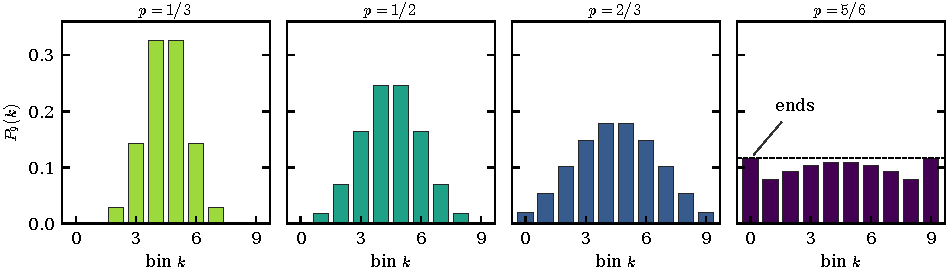
\includegraphics{figures/row10}
\caption{The bin probabilities $P_9(k)$ of Kagey's tenth row. At $p=5/6$, just
above $p_9$, the two middle bins are slightly below the ends (dashed line).}
\label{fig:row10}
\end{figure}

\begin{table}[ht]
\centering\small
\begin{tabular}{@{}rl@{\hskip 2em}rl@{\hskip 2em}rl@{\hskip 2em}rl@{}}
\toprule
$N$ & $p_N$ & $N$ & $p_N$ & $N$ & $p_N$ & $N$ & $p_N$\\
\midrule
2 & 0.66666667 & 6 & 0.78871211 & 10 & 0.83840411 & 50 & 0.94200405\\
3 & 0.70710678 & 7 & 0.80361731 & 11 & 0.84652725 & 100 & 0.96496633\\
4 & 0.74487450 & 8 & 0.81759938 & 12 & 0.85426060 & 200 & 0.97939018\\
5 & 0.76759188 & 9 & 0.82829163 & 20 & 0.89293837 & 400 & 0.98812464\\
\bottomrule
\end{tabular}
\caption{The value $p_N$ at which the middle and extreme bins of row $N+1$ are equally likely.}
\label{tab:pn}
\end{table}

The Bessel functions come in because the runs are long. When $Nu$ is about $\log N$, a typical
word only switches about $\log N$ times. Then the number of ways to split $a$ letters into $r$
runs, $\binom{a-1}{r}$, is close to $a^r/r!$, and after this change the run count is exactly the
power series of $I_0$ and $I_1$. The next theorem bounds the error we make by doing this.

\begin{theorem}[uniform Bessel approximation]\label{thm:bessel}
Put $h=N/2$, $J(x)=I_0(2x)+I_1(2x)$ and $F(x)=2xJ(x)$.
For every $N\ge2$ and $x>0$,
\begin{equation}\label{eq:uniformbessel}
0\le1-\frac{hS_N(x/h)}{F(x)}\le\frac{x(x+1)}h.
\end{equation}
Let $x_B$ be the unique positive root of $F(x_B)=h$, and put
$u_B=x_B/h$, $u_N=(1-p_N)/p_N$. Then
\[
0\le u_N-u_B=O((\log N)^2/N^2).
\]
Writing $L=\log N$ and $c_0=\tfrac12\log(\pi/8)$, we have
\begin{align}
N(1-p_N)&=L-\tfrac12\log L+c_0
+O\left(\frac{\log L}{L}\right),\label{eq:secondorder}\\
N(1-p_N)&=L-\tfrac12\log L+c_0
+\frac{\tfrac14\log L-\tfrac12c_0+\tfrac18}{L}
+O\left(\frac{(\log L)^2}{L^2}\right).\label{eq:thirdorder}
\end{align}
\end{theorem}
\begin{proof}
Let $a=\lfloor N/2\rfloor$, $b=\lceil N/2\rceil$, and define
\[
A_r=\frac{r!}{h^r}\binom{a-1}{r},\qquad
B_r=\frac{r!}{h^r}\binom{b-1}{r}\quad(r\ge0).
\]
With $(v)_+=\max(v,0)$, these have the product expressions
\[
A_r=\prod_{k=1}^r\left(1-\frac{h-a+k}{h}\right)_+,
\qquad B_r=\prod_{k=1}^r\left(1-\frac{h-b+k}{h}\right)_+.
\]
They lie in $[0,1]$, including beyond their finite support, where a factor is zero.
For nonnegative $t_j$, the inequality $1-\prod_j(1-t_j)_+\le\sum_jt_j$
holds even when some $t_j>1$. Since $a+b=2h$, it gives
\[
0\le1-A_rB_r\le\frac{r(r+1)}h.
\]
The deficits for $A_{r+1}B_r$ and $A_rB_{r+1}$ are at most
$((r+1)^2+h-a)/h$ and $((r+1)^2+h-b)/h$, respectively. Averaging cancels
the parity offsets, so
\[
0\le1-\frac{A_{r+1}B_r+A_rB_{r+1}}2\le\frac{(r+1)^2}h.
\]
The run-count formula, with $u=x/h$, becomes
\[
S_N(u)=2u\left[\sum_{r\ge0}\frac{x^{2r}}{(r!)^2}A_rB_r
+\sum_{r\ge0}\frac{x^{2r+1}}{r!(r+1)!}
\frac{A_{r+1}B_r+A_rB_{r+1}}2\right].
\]
Dropping the $A,B$ factors yields $2uJ(x)=F(x)/h$, using the Bessel series
\cite[Eq.~10.25.2]{dlmf}. Index shifts in those absolutely convergent series give
\begin{align*}
\sum_{r\ge0}r(r+1)\frac{x^{2r}}{(r!)^2}&=x^2I_0(2x)+xI_1(2x),\\
\sum_{r\ge0}(r+1)^2\frac{x^{2r+1}}{r!(r+1)!}&=x^2I_1(2x)+xI_0(2x).
\end{align*}
Their sum is $x(x+1)J(x)$, proving \eqref{eq:uniformbessel}, including the tail
beyond the finite polynomial support. In particular the relative error is
$O((\log N)^2/N)$ uniformly for $0<x\le C\log N$ for each fixed $C$.

Now let $x_N=hu_N$. Theorem~\ref{thm:root} gives $x_N\sim\tfrac12\log N$.
Differentiation gives $F'(x)=2F(x)+2I_0(2x)$, hence $F'/F\ge2$.
Set $\delta_N=x_N(x_N+1)/h$. For large $N$, $\delta_N<1$, and
\eqref{eq:uniformbessel} at the root gives
\[
h\le F(x_N)\le\frac{h}{1-\delta_N},\qquad
0\le x_N-x_B\le-\tfrac12\log(1-\delta_N)
=O((\log N)^2/N).
\]
Divide by $h$ for the assertion about $u$. Moreover,
\[
N(1-p_N)=\frac{2x_N}{1+x_N/h}=2x_B+O((\log N)^2/N).
\]
Put $z=2x_B$. The standard large-argument expansion
\cite[Eq.~10.40.1]{dlmf} is
\[
I_0(z)+I_1(z)=\frac{2e^z}{\sqrt{2\pi z}}
\left(1-\frac1{8z}+O(z^{-2})\right).
\]
Since $z(I_0(z)+I_1(z))=N/2$, taking logarithms gives
\[
z+\tfrac12\log z=L+c_0+\frac1{8z}+O(z^{-2}).
\]
First $z=L+O(\log L)$, then substitution proves \eqref{eq:secondorder}.
For one further term put $z=L+d+e/L$, where $d=-\tfrac12\log L+c_0$.
Matching coefficients of $1/L$ gives $e=\tfrac18-d/2$. The residual is
$O((\log L)^2/L^2)$. The derivative of $z+\tfrac12\log z$ is at least one, so
inverting keeps that order. This proves \eqref{eq:thirdorder}.
\end{proof}

The ratios $u_B/u_N$ are $0.9761$, $0.9864$, $0.9924$ at $N=100,200,400$ and
$0.99579$, $0.99769$, $0.99874$ at $N=800,1600,3200$. We predicted intervals for
the last three before computing them (\texttt{data/ledger.md}), and
Theorem~\ref{thm:bessel} proves the approximation behind those predictions.
Figure~\ref{fig:crossing} compares the exact roots with these approximations
up to $N=10^4$.

\begin{figure}[t]
\centering
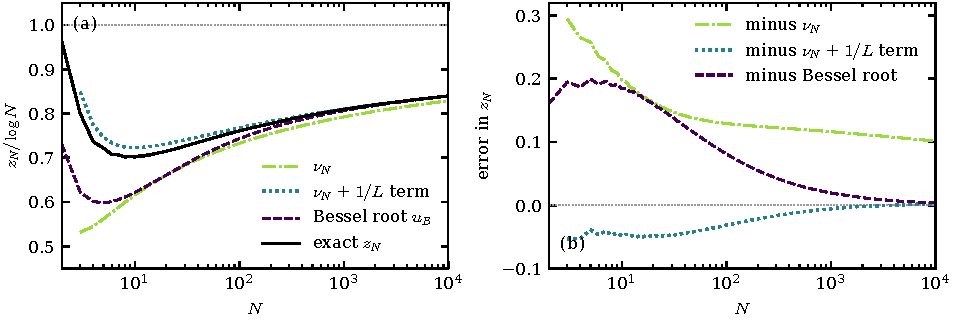
\includegraphics{figures/crossing}
\caption{(a) The scaled crossing $N(1-p_N)/\log N$ from the exact roots, from
the Bessel root $u_B$, and from the expansions \eqref{eq:secondorder} and
\eqref{eq:thirdorder} without their error terms. It tends to $1$ very slowly.
(b) The error of each approximation to $N(1-p_N)$.}
\label{fig:crossing}
\end{figure}

\begin{proposition}[adjacent bins and global extrema]\label{prop:adjacent}
For $N\ge2$ and $0<p<1$, an adjacent bin has the same probability as an endpoint precisely at
\[
p_N^{\mathrm{adj}}=\frac{1+\sqrt{N-1}}{2+\sqrt{N-1}}.
\]
For $0<p<1$, the endpoints are the least likely bins if $p<p_N^{\mathrm{adj}}$, bins
$1$ and $N-1$ are if $p>p_N^{\mathrm{adj}}$, and they tie at equality.
For $N\ge4$, the central crossing satisfies $p_N>p_N^{\mathrm{adj}}$.
At $p=p_N$, the middle and endpoints attain the global maximum and bins
$1,N-1$ attain the global minimum. For $N=2,3$,
$p_N=p_N^{\mathrm{adj}}$ and every bin ties at the crossing.
\end{proposition}
\begin{proof}
A word with one $R$ has one change in two cases and two changes in $N-2$ cases.
Thus $P_N(1)/P_N(0)=2u+(N-2)u^2$, whose positive root at level one is
$u^{\mathrm{adj}}=1/(1+\sqrt{N-1})$, including $N=2$.
This yields the stated $p$ and sign change.
By Proposition~\ref{prop:allbin-order} in Section~\ref{sec:allbin}, which we prove from the
run-count formula, the interior bins get more likely as we move toward the middle. By
symmetry, the middle is then the largest interior bin and bins $1$ and $N-1$ are the smallest.
Comparing bins $1,N-1$ with the endpoints gives the claims about the global minimum.

Put $a=\lfloor N/2\rfloor$ and $b=\lceil N/2\rceil$.
The polynomial $S_N(u)$ begins with $2u+(N-2)u^2$ and has
nonnegative coefficients. For $N\ge4$, its cubic coefficient is
$2(a-1)(b-1)>0$. Consequently, at its positive root $u_N$,
\[
 2u_N+(N-2)u_N^2<S_N(u_N)=1.
\]
The adjacent polynomial is strictly increasing, so $u_N<u^{\mathrm{adj}}$
and hence $p_N>p_N^{\mathrm{adj}}$. The middle and endpoints tie by
definition of $p_N$, proving the global-maximum assertion as well.
For $N=2,3$, $S_N(u)=2u+(N-2)u^2$, and symmetry gives the stated ties.
In particular $p_3=p_3^{\mathrm{adj}}=1/\sqrt2$.
\end{proof}

The adjacent-bin scale is $1-p_N^{\mathrm{adj}}\sim N^{-1/2}$, distinct from
$1-p_N\sim(\log N)/N$. This makes sense. Bin $1$ has a single $R$, and unless it is at one of
the ends it needs two switches. So $P_N(1)/P_N(0)\approx Nu^2$, which only reaches $1$ at
$u\approx N^{-1/2}$. The middle bin has far more words, so it catches up to the endpoints much
earlier. At $p=0,1$ there are also ties between bins of probability zero.

\section{The full hierarchy of endpoint crossings}\label{sec:allbin}

Let $a,b\ge1$ be integers, $N=a+b$, $u=(1-p)/p$ with $p>0$, and
$S_{a,b}(u)=P_N(a)/P_N(0)$. Theorem~\ref{thm:pmf} and
$\binom{m-1}{r+1}=\frac{m-1-r}{r+1}\binom{m-1}{r}$ for $m=a,b$ give
\begin{equation}\label{eq:allbin-polynomial}
 S_{a,b}(u)=\sum_{r\ge0}\binom{a-1}{r}\binom{b-1}{r}
 \Bigl(2u^{2r+1}+\frac{N-2-2r}{r+1}u^{2r+2}\Bigr).
\end{equation}
Its coefficients are nonnegative, as $N-2-2r\ge|b-a|$ for $r<\min(a,b)$,
and the linear one is $2$. So there is a unique $u_{a,b}>0$ with
$S_{a,b}(u_{a,b})=1$, and we put $p_{a,b}=1/(1+u_{a,b})$. As $S_{a,b}(u)\ge2u$,
$u_{a,b}\le\frac12$ and $p_{a,b}\in[\frac23,1)$, with $p_{a,b}=\frac23$ only for
$a=b=1$.

\begin{proposition}[ordering the crossings]\label{prop:allbin-order}
If $a<b-1$, then
\[
 u_{a+1,b-1}<u_{a,b},\qquad p_{a+1,b-1}>p_{a,b}.
\]
Also $p_{a,b+1}>p_{a,b}$ for all positive $a,b$.
In fact, the corresponding inequalities between the polynomials
$S_{a+1,b-1}$ and $S_{a,b}$, or $S_{a,b+1}$ and $S_{a,b}$, hold
coefficientwise, with at least one strict coefficient.
\end{proposition}
\begin{proof}
For fixed $N$ and $r\le a-1$,
$\binom{a-1}{r}\binom{b-1}{r}=(r!)^{-2}\prod_{j=0}^{r-1}(a-1-j)(b-1-j)$, and
each factor grows when $(a,b)$ becomes $(a+1,b-1)$, by
$(a-j)(b-2-j)-(a-1-j)(b-1-j)=b-a-1>0$. The even multiplier $(N-2-2r)/(r+1)$
is unchanged, and nonnegative where either product is nonzero, since then
$r\le a$ and $N-2-2r\ge b-a-2\ge0$. New summands are nonnegative, and the
cubic coefficient grows strictly. Increasing $b$ with $a$
fixed increases the binomial coefficients of Theorem~\ref{thm:pmf}, and the
quadratic coefficient $N-2$ strictly. Comparing the unique roots proves the rest.
\end{proof}

The ordering of the bin heights below also follows from the interior
log-concavity of Dekking and Kong~\cite[Proposition~4.3]{dekkingkong2011}.
We use the coefficients.

\begin{proposition}[adjacent bins and global extrema]\label{prop:adjacent}
For $N\ge2$ and $0<p<1$, an adjacent bin has the same probability as an endpoint precisely at
\[
p_N^{\mathrm{adj}}=\frac{1+\sqrt{N-1}}{2+\sqrt{N-1}}.
\]
For $0<p<1$, the endpoints are the least likely bins if $p<p_N^{\mathrm{adj}}$, bins
$1$ and $N-1$ are if $p>p_N^{\mathrm{adj}}$, and they tie at equality.
For $N\ge4$, the central crossing satisfies $p_N>p_N^{\mathrm{adj}}$.
At $p=p_N$, the middle and endpoints attain the global maximum and bins
$1,N-1$ attain the global minimum. For $N=2,3$,
$p_N=p_N^{\mathrm{adj}}$ and every bin ties at the crossing.
\end{proposition}
\begin{proof}
By \eqref{eq:allbin-polynomial}, $S_{1,N-1}(u)=2u+(N-2)u^2$, with positive root
$u^{\mathrm{adj}}=1/(1+\sqrt{N-1})$. This gives $p_N^{\mathrm{adj}}$ and the sign
change. For $0<p<1$ we have $P_N(k)=P_N(0)S_{k,N-k}(u)$ with $P_N(0)>0$, so if
$1\le k<N-k-1$ Proposition~\ref{prop:allbin-order} gives $P_N(k)<P_N(k+1)$. By
symmetry the middle is the largest interior bin and bins $1,N-1$ are the
smallest, which gives the claims about the global minimum. For $N\ge4$ the
cubic coefficient $2(\lfloor N/2\rfloor-1)(\lceil N/2\rceil-1)$ of $S_N$ is
positive, so $2u_N+(N-2)u_N^2<S_N(u_N)=1$, hence $u_N<u^{\mathrm{adj}}$ and
$p_N>p_N^{\mathrm{adj}}$. At $p_N$ the middle ties with the endpoints, which
gives the global maximum. For $N=2,3$ we have $S_N=S_{1,N-1}$, and symmetry
gives the ties.
\end{proof}

So $1-p_N^{\mathrm{adj}}\sim N^{-1/2}$, much larger than $1-p_N\sim(\log N)/N$.
Away from the ends the single $\sR$ of bin $1$ needs $2$ switches, so
$S_{1,N-1}\approx Nu^2$ reaches $1$ only at $u\approx N^{-1/2}$ (at $p=0,1$
there are also ties between bins of probability $0$).

\subsection{A Bessel estimate uniform in the bin}

Bin $a$ has about $(a^r/r!)(b^r/r!)$ words with $r$ runs of each letter, each
of weight about $u^{2r}$. The sum depends only on $abu^2$, so a bin near the
edge acts like the middle of a shorter row with $\sqrt{ab}$ in place of $N/2$.
Put
\[
 s=\sqrt{ab},\quad A=\frac{ab}{a+b},\quad
 c=\frac{a+b}{2\sqrt{ab}},\quad
 \eta=\frac1c,\quad x=su,\quad J_c(x)=I_0(2x)+cI_1(2x),
\]
and $\widehat S_{a,b}(u)=2uJ_c(su)$.

\begin{theorem}[uniform estimate for every bin]\label{thm:allbin-bessel}
For all positive integers $a,b$ and all $u>0$,
\begin{equation}\label{eq:allbin-bessel}
 0\le 1-\frac{S_{a,b}(u)}{\widehat S_{a,b}(u)}
 \le \frac{(a+b)u^2}{2}+u
 =\frac{x^2}{2A}+\frac xs.
\end{equation}
In particular, for fixed $N$ and $u$ the bound does not depend on the bin.
The inequality still holds when the right side exceeds 1, but then it
gives no lower bound on $S_{a,b}$.
\end{theorem}
\begin{proof}
Let $U_r=U_r(a)$ and $V_r=U_r(b)$ as in Lemma~\ref{lem:clipped}(b), and
$H=1/a+1/b=1/A$. Lemma~\ref{lem:clipped}(a), applied to the $2r$ clipped
factors of $U_rV_r$, gives
\begin{equation}\label{eq:allbin-odd-deficit}
 0\le1-U_rV_r\le\frac H2r(r+1).
\end{equation}
The same argument for $E_r=(aU_{r+1}V_r+bU_rV_{r+1})/(a+b)$ gives
\begin{align}
 0\le1-E_r
 &\le\frac{(r+1)(r+2)}{a+b}
 +\frac{r(r+1)}{2(a+b)}\Bigl(\frac ab+\frac ba\Bigr)\notag\\
 &=\frac H2r(r+1)+\frac{2(r+1)}{a+b}.\label{eq:allbin-even-deficit}
\end{align}
Since $\binom{a-1}r=a^rU_r/r!$, \eqref{eq:allbin-polynomial} becomes
\begin{equation}\label{eq:allbin-normalized-series}
 S_{a,b}(u)=2u\Bigl[
 \sum_{r\ge0}\frac{x^{2r}}{(r!)^2}U_rV_r
 +c\sum_{r\ge0}\frac{x^{2r+1}}{r!(r+1)!}E_r\Bigr],
\end{equation}
and dropping $U_rV_r$ and $E_r$ gives $\widehat S_{a,b}(u)$. So by
Lemma~\ref{lem:clipped}(c), with $I_j=I_j(2x)$,
$(\widehat S_{a,b}-S_{a,b})/(2u)$ lies between $0$ and
\[
 \frac H2(x^2I_0+xI_1+cx^2I_1)+\frac{2c\,xI_0}{a+b}
 =\Bigl(\frac{x^2}{2A}+\frac xs\Bigr)J_c(x),
\]
since $H/2=c/s=1/(2A)$ and $2c/(a+b)=1/s$.
\end{proof}

Let $x_{a,b}=su_{a,b}$ and let $x_B$ be the positive root of
\begin{equation}\label{eq:allbin-bessel-root}
 G_\eta(x_B)=A,\qquad
 G_\eta(x)=x\{I_1(2x)+\eta I_0(2x)\}.
\end{equation}
Differentiating term by term gives
\begin{equation}\label{eq:allbin-logderivative}
 G_\eta'(x)-2G_\eta(x)
 =2x(1-\eta)\{I_0(2x)-I_1(2x)\}+\eta I_0(2x)\ge0,
\end{equation}
since $I_0(2x)-I_1(2x)=\frac1\pi\int_0^\pi e^{2x\cos\theta}(1-\cos\theta)\,d\theta>0$
by \cite[Eq.~10.32.3]{dlmf}. So $(\log G_\eta)'\ge2$ for $x>0$ and
$0\le\eta\le1$.

\begin{corollary}[quantitative crossing bound]\label{cor:allbin-root-bound}
We have $x_{a,b}\ge x_B$. If
\[
 \delta_{a,b}=\frac{x_{a,b}^2}{2A}+\frac{x_{a,b}}s<1,
\]
then
\begin{equation}\label{eq:allbin-root-bound}
 0\le x_{a,b}-x_B\le-\tfrac12\log(1-\delta_{a,b}).
\end{equation}
\end{corollary}
\begin{proof}
Since $c\eta=1$ and $2c/s=1/A$, we have $\widehat S_{a,b}(u)=G_\eta(su)/A$. At
the crossing $S_{a,b}=1$, so Theorem~\ref{thm:allbin-bessel} gives
$A\le G_\eta(x_{a,b})\le A/(1-\delta_{a,b})$. As $G_\eta(x_B)=A$, this gives
$x_{a,b}\ge x_B$, and integrating $(\log G_\eta)'\ge2$ from $x_B$ to $x_{a,b}$
gives \eqref{eq:allbin-root-bound}. For $\eta=1$, where $2G_1=F$, this is the
proof of Theorem~\ref{thm:bessel}(ii).
\end{proof}

\begin{remark}[Jacobi polynomials]\label{rem:jacobi}
The Bessel forms in this paper come from the confluence of Jacobi, Laguerre
and Bessel functions near the point $1$. For $a\le b$ and $0\le t<1$,
\[
 \sum_{r\ge0}\binom{a-1}{r}\binom{b-1}{r}t^r
 ={}_2F_1(1-a,1-b;1;t)
 =(1-t)^{a-1}P_{a-1}^{(0,\,b-a)}\Bigl(\frac{1+t}{1-t}\Bigr),
\]
and for $b>a$ and $0\le u<1$,
\[
 \sum_{r\ge0}\binom{a-1}{r}\binom{b-1}{r+1}u^{2r+2}
 =\frac{(b-1)u^2}{a}(1-u^2)^{a-1}P_{a-1}^{(1,\,b-a-1)}\Bigl(\frac{1+u^2}{1-u^2}\Bigr).
\]
Near $1$, Jacobi polynomials of large degree behave like Bessel functions
(the Mehler--Heine formula \cite[Eq.~18.11.5]{dlmf}), and Elliott~\cite{elliott1971}
gives expansions in modified Bessel functions uniform near $1$. For fixed $a$
and $y=bu^2$, as $b\to\infty$, \cite[Eq.~18.7.21]{dlmf} turns the last sum into
$(y/a)L_{a-1}^{(1)}(-y)=H_a(y)$ of \eqref{eq:edge-polynomial}, and the other
terms tend to $0$. Temme~\cite{temme1990} gives asymptotic estimates of
Gegenbauer, Laguerre and Jacobi polynomials. These forms are classical. But Elliott's expansions
have fixed parameters and no error bounds, while here $b-a$ can be as large as
$N-2$, and Theorem~\ref{thm:allbin-bessel} gives an explicit relative error at
every $N$.
\end{remark}

\begin{lemma}[inverting $z+\frac12\log z$]\label{lem:inversion}
Fix $K>0$. Let $z\ge1$ and $\ell\ge2$, and suppose that
$z+\tfrac12\log z=\ell+C+B/z+\omega$ with $|C|,|B|\le K$ and $|\omega|\le1$. Then
\[
z=\ell-\tfrac12\log\ell+C+\frac{\frac14\log\ell-\frac12C+B}{\ell}
+O_K\Bigl(\frac{(\log\ell)^2}{\ell^2}+|\omega|\Bigr).
\]
\end{lemma}
\begin{proof}
Put $w=z-\ell$. As $z\ge1$, $\log z\ge0$ and $|B/z|\le K$, so $z\le\ell+2K+1$
and $|w|\le2K+1+\frac12\log(\ell+2K+1)=O_K(\log\ell)$, proving the claim for
$\ell$ bounded in terms of $K$. For larger $\ell$, $|w|\le\ell/2$, so
$\log z=\log\ell+w/\ell+O((w/\ell)^2)$ and $B/z=B/\ell+O_K(|w|/\ell^2)$, and
$w=C-\frac12\log\ell-w/(2\ell)+B/\ell+\omega+O_K((\log\ell)^2/\ell^2)$. This
gives first $w=d+O_K(\log\ell/\ell+|\omega|)$ with $d=C-\frac12\log\ell$, and
then $w=d+(B-d/2)/\ell+O_K((\log\ell)^2/\ell^2+|\omega|)$.
\end{proof}

\subsection{Every growing distance from an edge}

\begin{theorem}[uniform crossing expansion]\label{thm:allbin-expansion}
Suppose $1\le a\le b$ and $a\to\infty$, with no restriction on the relative
growth of $a$ and $b$. Put
\[
 \ell=\log A,\qquad
 C(\eta)=\tfrac12\log(8\pi)-\log(1+\eta),\qquad
 B(\eta)=\frac{3-\eta}{8(1+\eta)}.
\]
Uniformly over $b\ge a$,
\begin{align}
 2\sqrt{ab}\,u_{a,b}
 ={}&\ell-\tfrac12\log\ell+C(\eta)\notag\\
 &+\frac{\tfrac14\log\ell-\tfrac12C(\eta)+B(\eta)}{\ell}
 +O\left(\frac{(\log\ell)^2}{\ell^2}+\frac{(\log a)^2}{a}\right).
 \label{eq:allbin-expansion}
\end{align}
The same expansion and error order hold with $1-p_{a,b}$ in place of $u_{a,b}$.
\end{theorem}
\begin{proof}
Here $a/2\le A\le a$, $s\ge a$ and $0<\eta\le1$. At $x=\log a$ the bound
of Theorem~\ref{thm:allbin-bessel} is at most $2(\log a)^2/a$, while
$G_\eta(x)/A\ge xI_1(2x)/a\to\infty$. So $S_{a,b}>1$ there, $x_{a,b}\le\log a$
for large $a$, uniformly in $b$, and Corollary~\ref{cor:allbin-root-bound} gives
\begin{equation}\label{eq:allbin-root-error}
 x_{a,b}-x_B=O((\log a)^2/a).
\end{equation}
Write $z=2x_B$, so $z\to\infty$ as $A\to\infty$. By
\cite[Eq.~10.40.1]{dlmf},
$I_1(z)+\eta I_0(z)=(1+\eta)e^z(2\pi z)^{-1/2}(1-B(\eta)/z+O(z^{-2}))$
uniformly in $0\le\eta\le1$, so \eqref{eq:allbin-bessel-root} becomes
$z+\frac12\log z=\ell+C(\eta)+B(\eta)/z+O(z^{-2})$. As $|C(\eta)|\le2$ and
$0<B(\eta)\le\frac38$, Lemma~\ref{lem:inversion} expands $z$, and
\eqref{eq:allbin-root-error} moves this to $2x_{a,b}=2\sqrt{ab}\,u_{a,b}$.
Finally $2s(u-u/(1+u))\le2x^2/s=O((\log a)^2/a)$ at $u=u_{a,b}$.
\end{proof}

Hence, uniformly in $b$,
\begin{equation}\label{eq:allbin-leading}
 1-p_{a,b}\sim\frac{\log a}{2\sqrt{ab}}
 \qquad(a\to\infty,\ b\ge a).
\end{equation}
If $a=o(b)$, then $\eta\to0$ and $\log A=\log a+o(1)$, so
\begin{equation}\label{eq:allbin-growing-edge}
 2\sqrt{ab}(1-p_{a,b})
 =\log a-\tfrac12\log\log a+\tfrac12\log(8\pi)+o(1).
\end{equation}
If $a/N\to\alpha\in(0,\frac12]$ at any rate, then
\[
 2\sqrt{a(N-a)}(1-p_{a,N-a})
 =\log N-\tfrac12\log\log N+\log\{\alpha(1-\alpha)\}+C(2\sqrt{\alpha(1-\alpha)})+o(1).
\]
At the center, $a=b=N/2$ gives $A=N/4$ and $\eta=1$, and changing from
$\log A$ to $\log N$ recovers \eqref{eq:thirdorder}.

\begin{figure}[t]
\centering
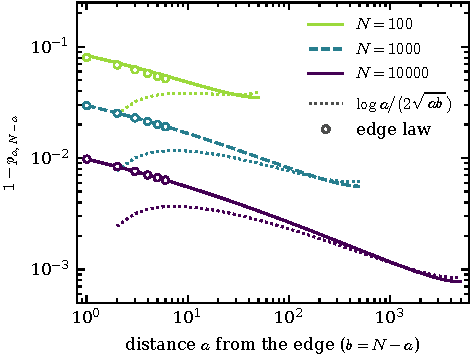
\includegraphics{figures/allbin}
\caption{The crossing $1-p_{a,N-a}$ of each bin against its distance $a$
from the nearer edge, for $N=100$, $1000$ and $10^4$. The dotted lines are the
leading law \eqref{eq:allbin-leading}, and the circles are the edge law
\eqref{eq:edge-q-expansion} for $a\le6$. The right end of each line is the
central crossing $1-p_N$.}
\label{fig:allbin}
\end{figure}

\subsection{Fixed bins and the Laguerre edge law}

If $a$ is fixed and $b\to\infty$, each run of $\sR$'s away from the ends needs
$2$ switches, giving $u^2$, and can go in about $b$ places. So we use
$y=bu^2$. Define
\begin{equation}\label{eq:edge-polynomial}
 H_a(y)=\sum_{r=0}^{a-1}\binom{a-1}{r}\frac{y^{r+1}}{(r+1)!}
 =\frac ya L_{a-1}^{(1)}(-y),
\end{equation}
with the standard Laguerre polynomial $L_{a-1}^{(1)}$.
Let $y_a$ be the positive root of $H_a(y_a)=1$ and $c_a=\sqrt{y_a}$. Then
$y_1=1$, $y_2=\sqrt3-1$, and $y_a$ decreases strictly in $a$, by coefficient
comparison.

\begin{theorem}[fixed-edge expansion]\label{thm:edge-laguerre}
For each fixed positive integer $a$, as $b\to\infty$,
\begin{equation}\label{eq:edge-crossing-expansion}
 u_{a,b}=\frac{c_a}{\sqrt b}-\frac1b
 +\frac{\gamma_a}{b^{3/2}}+O_a(b^{-2}),
\end{equation}
where
\[
 \gamma_a=
 \frac{1+y_a+(y_a+y_a^2/2)H_a''(y_a)/H_a'(y_a)}{2c_a}.
\]
Thus the second coefficient in the odds expansion is $-1$ for every fixed
bin. For the switching probability,
\begin{equation}\label{eq:edge-q-expansion}
 1-p_{a,b}=\frac{c_a}{\sqrt b}-\frac{1+c_a^2}{b}+O_a(b^{-3/2}).
\end{equation}
\end{theorem}
\begin{proof}
Put $\epsilon=b^{-1/2}$, $y=bu^2$ and $V_r=U_r(b)$. For $b\ge a$,
\eqref{eq:allbin-polynomial} reads
\begin{align}
 S_{a,b}(u)={}&2\sqrt{y/b}\sum_r\binom{a-1}{r}\frac{y^r}{r!}V_r\notag\\
 &+\frac yb\sum_r\binom{a-1}{r+1}\frac{y^r}{r!}V_r
 +y\sum_r\binom{a-1}{r}\frac{y^r}{(r+1)!}V_{r+1}.
 \label{eq:edge-exact-series}
\end{align}
These sums have at most $a$ terms, and with $V_r=1$ they are $H_a'(y)$,
$H_a''(y)$ and $H_a(y)$. Expanding $V_r=1-r(r+1)/(2b)+O_a(b^{-2})$ and using
$\sum_r(r+1)(r+2)\binom{a-1}{r}\frac{y^{r+1}}{(r+1)!}=y^2H_a''(y)+2yH_a'(y)$
gives, uniformly near $y=y_a$,
\begin{align}
 S_{a,b}(u)={}&H_a(y)+2\sqrt y\,H_a'(y)\epsilon\notag\\
 &+\{(y-y^2/2)H_a''(y)-yH_a'(y)\}\epsilon^2+O_a(\epsilon^3).
 \label{eq:edge-implicit-expansion}
\end{align}
With $b=\epsilon^{-2}$ the right side of \eqref{eq:edge-exact-series} is
analytic in $(\epsilon,y)$ near $(0,y_a)$, and $H_a'(y_a)>0$. So the
implicit-function theorem and the uniqueness of the crossing give
$y=y_a+d_1\epsilon+d_2\epsilon^2+O_a(\epsilon^3)$ at $u=u_{a,b}$, and matching
coefficients in \eqref{eq:edge-implicit-expansion} gives $d_1=-2c_a$ and
$d_2=2+y_a+(y_a+y_a^2/2)H_a''(y_a)/H_a'(y_a)$. Expanding $u=\epsilon\sqrt y$
and then $u/(1+u)$ proves both expansions.
\end{proof}

\begin{theorem}[matching the edge and Bessel regimes]\label{thm:edge-matching}
For every positive integer $a$ and every $x>0$,
\begin{equation}\label{eq:laguerre-bessel-bound}
 0\le1-\frac{aH_a(x^2/a)}{xI_1(2x)}\le\frac{x^2}{2a}.
\end{equation}
Consequently, with $\ell=\log a$ and $C_0=\tfrac12\log(8\pi)$,
\begin{align}
 2\sqrt{a y_a}
 ={}&\ell-\tfrac12\log\ell+C_0\notag\\
 &+\frac{\tfrac14\log\ell-\tfrac12C_0+3/8}{\ell}
 +O\left(\frac{(\log\ell)^2}{\ell^2}+\frac{(\log a)^2}{a}\right).
 \label{eq:edge-matching-expansion}
\end{align}
\end{theorem}
\begin{proof}
With $U_r=U_r(a)$, $aH_a(x^2/a)=x\sum_{r\ge0}U_rx^{2r+1}/(r!(r+1)!)$, so
Lemma~\ref{lem:clipped}(b) and the second identity of
Lemma~\ref{lem:clipped}(c) give \eqref{eq:laguerre-bessel-bound}. Put
$x_a=\sqrt{ay_a}$, so $aH_a(x_a^2/a)=a$, and $x_a<\log a$ for large $a$ by
\eqref{eq:laguerre-bessel-bound}. So $a\le G_0(x_a)\le a/(1-x_a^2/(2a))$, and as in
Corollary~\ref{cor:allbin-root-bound},
$x_a-x_0=O((\log a)^2/a)$, where $G_0(x_0)=a$. So $z=2x_0$ satisfies
$z+\frac12\log z=\ell+C_0+3/(8z)+O(z^{-2})$ by \cite[Eq.~10.40.1]{dlmf}, as in
the proof of Theorem~\ref{thm:allbin-expansion} with $\eta=0$, $A=a$, and
Lemma~\ref{lem:inversion} gives the expansion.
\end{proof}

Figure~\ref{fig:allbin} compares these laws with the exact crossings.

\subsection{The moving boundary layer}

The all-bin expansion also gives the shape of a row at odds $u=v_N>0$. Let
\[
 \mathcal L_N=\#\{1\le k\le\lfloor N/2\rfloor:P_N(k)<P_N(0)\}.
\]
\begin{corollary}[boundary-layer width]\label{cor:boundary-layer}
Suppose
\[
 \Omega_N=\frac1{\sqrt N\,v_N}\longrightarrow\infty,
 \qquad \frac{\log\Omega_N}{Nv_N}\longrightarrow0.
\]
Then
\begin{equation}\label{eq:boundary-layer-width}
 \mathcal L_N\sim\Omega_N^2\log^2\Omega_N
 =\frac{\log^2(1/(\sqrt N\,v_N))}{Nv_N^2}.
\end{equation}
In particular, if $v_N=N^{-\gamma}$ with $1/2<\gamma<1$, then
\[
 \mathcal L_N\sim(\gamma-\tfrac12)^2N^{2\gamma-1}\log^2N.
\]
By symmetry, the total number of interior bins below the endpoint height
is $2\mathcal L_N$ for all sufficiently large $N$.
\end{corollary}
\begin{proof}
Set $d_N=\Omega_N^2\log^2\Omega_N$. Then $d_N\to\infty$ and
$d_N/N=(\log\Omega_N/(Nv_N))^2\to0$. Fix $\varepsilon\in(0,1)$ and integers
$a_\pm=(1\pm\varepsilon)d_N+O(1)$. Then $\log a_\pm\sim2\log\Omega_N$ and
$\sqrt{a_\pm(N-a_\pm)}\,v_N\sim\sqrt{1\pm\varepsilon}\,\log\Omega_N$, so
Theorem~\ref{thm:allbin-expansion} gives $u_{a_\pm,N-a_\pm}/v_N\to1/\sqrt{1\pm\varepsilon}$.
Bin $k$ is below the endpoint exactly when $v_N<u_{k,N-k}$, and $u_{k,N-k}$
decreases strictly for $k\le N/2$ by Proposition~\ref{prop:allbin-order}. So
$a_-\le\mathcal L_N<a_+$ for large $N$, and we let $\varepsilon\downarrow0$.
Finally $\mathcal L_N=o(N)$, so the
reflected intervals are disjoint.
\end{proof}

\section{Boundary conditions and a spatial crossing window}\label{sec:periodicwindow}

The binary model is also a zero-field Ising chain with free boundaries. For step signs
$\varepsilon_i\in\{-1,1\}$ its weight is proportional to
$\exp(K\sum_{i=1}^{N-1}\varepsilon_i\varepsilon_{i+1})$, where
$u=q/p=e^{-2K}$. The analogous periodic measure includes the last-to-first bond.
Antal, Droz and R\'acz~\cite{antal2004} derive boundary-dependent limiting magnetization
laws, and Dantchev and Rudnick~\cite{dantchev2022} give exact free and periodic coefficients.
Stepanyan et al.~\cite{stepanyan2024} study the periodic endpoint--adjacent
and endpoint--center comparisons directly. So neither the periodic law nor the
crossing question is new. Here we bound the discrete error uniformly and give a
large-$N$ expansion that refines their finite-size approximation.

Note that the periodic spin measure is not the same as wrapping the free Galton walk
around a cylinder, which is the case in Remark~\ref{rem:cyl}.
Write $R^{\mathrm F}_{N,k}$ and $R^{\mathrm P}_{N,k}$ for bin-to-endpoint ratios under
free and periodic boundaries. Put $a=k$, $b=N-k$ and $s=\sqrt{ab}$. The classical cyclic count is
\begin{equation}\label{eq:periodicratio}
R^{\mathrm P}_{N,k}(u)=\sum_{r=1}^{\min(a,b)}\frac Nr
 \binom{a-1}{r-1}\binom{b-1}{r-1}u^{2r}.
\end{equation}
Indeed, choose compositions of each letter count into $r$ positive runs, choose a
labeled position for the start of a distinguished run of one letter, and divide by
its $r$ possible choices. The normalization of the periodic measure cancels in the ratio.
In particular $R^{\mathrm P}_{N,1}=Nu^2$, giving the known adjacent threshold
$K=(\log N)/4$. Every interior ratio is strictly increasing from zero to infinity in
$u>0$, and the ratios increase strictly toward the middle, except for the symmetric
middle-bin tie. The coefficient comparison uses the same products $(a-j)(b-j)$ as
the free case.

\begin{theorem}[periodic relative error]\label{thm:periodic-bessel}
For $N\ge2$, $1\le k\le N-1$, and $u>0$, define
\[
T^{\mathrm P}_{N,k}(u)=\frac{Nu}{\sqrt{k(N-k)}}
 I_1\!\left(2u\sqrt{k(N-k)}\right).
\]
Then
\begin{equation}\label{eq:periodicbound}
0\le1-\frac{R^{\mathrm P}_{N,k}(u)}{T^{\mathrm P}_{N,k}(u)}
\le\frac{Nu^2}{2}.
\end{equation}
\end{theorem}
\begin{proof}
Set $x=su$, $A=ab/N$, and
$U_r=r!\binom{a-1}{r}/a^r$, $V_r=r!\binom{b-1}{r}/b^r$.
The clipped-product inequality gives
$0\le1-U_rV_r\le r(r+1)/(2A)$, including the zero factors beyond support.
After shifting the index in \eqref{eq:periodicratio}, the ratio to $T^{\mathrm P}$ is
the weighted average of $U_rV_r$ with weights $x^{2r+1}/(r!(r+1)!)$.
Their sum is $I_1(2x)$, while their $r(r+1)$-weighted sum is $x^2I_1(2x)$.
Thus the relative deficit is at most $x^2/(2A)=Nu^2/2$.
\end{proof}

We can guess the $\log 2$ in the next theorem. A cyclic word always switches an even number of
times, but a free word can also start and end on different letters, and those words give the
$I_0$ term in the free approximation. For large arguments $I_0\approx I_1$, so near the crossing
the free ratio is about twice the periodic one. Both grow like $e^{Nu}$, so the periodic crossing
should need $Nu$ to be about $\log 2$ larger.

\begin{theorem}[periodic crossing and boundary shift]\label{thm:periodic-crossing}
Let $u_N^{\mathrm P}$ be the positive central root, and let $u_N^{\mathrm F}=u_N$
be the free central root. Put $L=\log N$ and $c_{\mathrm P}=\tfrac12\log(\pi/2)$.
Then
\begin{align}
Nu_N^{\mathrm P}
 &=L-\tfrac12\log L+c_{\mathrm P}
 +\frac{\tfrac14\log L-\tfrac12c_{\mathrm P}+\tfrac38}{L}
 +O\!\left(\frac{(\log L)^2}{L^2}\right),\label{eq:periodicasym}\\
N(u_N^{\mathrm P}-u_N^{\mathrm F})
 &=\log2+\frac{\tfrac14-\tfrac12\log2}{\log N}
 +o(1/\log N).\label{eq:boundaryshift}
\end{align}
Replacing $Nu_N^{\mathrm P}$ by $N(1-p_N^{\mathrm P})$ preserves
\eqref{eq:periodicasym}. In the Ising convention $K=\beta J$,
\begin{equation}\label{eq:isingtemperature}
\beta_N^{\mathrm P}J
=\tfrac12(\log N-\log\log N)
+\frac{\tfrac14\log\log N-\tfrac12c_{\mathrm P}}{\log N}
+O\!\left(\frac{(\log\log N)^2}{(\log N)^2}\right).
\end{equation}
\end{theorem}
\begin{proof}
At the middle, $2s=N+O(1/N)$. Evaluate Theorem~\ref{thm:periodic-bessel}
at $u=c\log N/N$ for fixed $c>0$. Its relative error tends to zero, and the Bessel
expansion makes the ratio tend to zero when $c<1$ and to infinity when $c>1$.
Monotonicity therefore gives $Nu_N^{\mathrm P}\sim\log N$.
Writing $z=Nu_N^{\mathrm P}$ and using
$I_1(z)=e^z(2\pi z)^{-1/2}(1-3/(8z)+O(z^{-2}))$ in the estimate at the root yields
\[
z+\tfrac12\log z=L+c_{\mathrm P}+\frac3{8z}
+O(z^{-2}+L^2/N).
\]
The odd-$N$ argument change contributes only $O(L/N^2)$ to this logarithmic equation.
Substitute $z=L+d+e/L$. The constant terms give
$d=-\tfrac12\log L+c_{\mathrm P}$, and the $1/L$ terms give $e=3/8-d/2$.
The derivative of the left side is at least one, so the residual yields the stated
error. Since $N(u-u/(1+u))=O(L^2/N)$, the switching-probability version follows.
Subtract the free expansion, where $c_{\mathrm F}=\tfrac12\log(\pi/8)$ and the
correction is $1/8$, to obtain \eqref{eq:boundaryshift}. Finally
$\beta J=-\tfrac12\log u=\tfrac12(L-\log z)$ gives \eqref{eq:isingtemperature}.
\end{proof}

Stepanyan et al.\ describe their formula \cite[Eq.~(16)]{stepanyan2024}, which is
linear in $\log N$, as a finite-size approximation. Equation~\eqref{eq:isingtemperature}
gives the large-$N$ behavior with a proved error term.

The factor $e^{-2y^2}$ is not hard to see. If we move $yN/\sqrt{\log N}$ away from the
middle, the Bessel argument is multiplied by $2\sqrt{k(N-k)}/N\approx1-2y^2/\log N$. The argument
is about $\log N$, so it goes down by about $2y^2$, and since the ratio grows roughly like $e$ to
the argument, it goes down by a factor of about $e^{-2y^2}$.

\begin{theorem}[spatial crossing window]\label{thm:critical-window}
Let $X\in\{\mathrm F,\mathrm P\}$ and let $u_N^X$ be its exact central crossing.
For fixed real $t,y$ set
\[
u=u_N^X+\frac tN,\qquad
k_N(y)=\operatorname{nint}\!\left(\frac N2+\frac{yN}{\sqrt{\log N}}\right),
\]
where either nearest-integer convention may be used. Then, uniformly on compact
sets of $(t,y)$,
\begin{equation}\label{eq:criticalprofile}
R^X_{N,k_N(y)}(u_N^X+t/N)\longrightarrow e^{t-2y^2}.
\end{equation}
If $M_N^X(t)$ is the number of interior bins with probability strictly above the
endpoint probability at that parameter, then
\begin{equation}\label{eq:criticalcount}
\frac{\sqrt{\log N}}N M_N^X(t)\longrightarrow\sqrt{2\max(t,0)}.
\end{equation}
\end{theorem}
\begin{proof}
Put $L=\log N$, $\delta=k/N-1/2$, and
$\eta=2\sqrt{k(N-k)}/N=\sqrt{1-4\delta^2}$.
For the stated rounding and bounded $y$,
\[
\eta=1-\frac{2y^2}{L}+O\!\left(L^{-2}+\frac1{N\sqrt L}\right),
\qquad Nu_N^X=L+O(\log L).
\]
Thus the Bessel argument at $(u,k)$ equals
$(Nu_N^X+t)\eta=Nu_N^X+t-2y^2+o(1)$, uniformly on the compact set.
Use the free all-bin estimate and Theorem~\ref{thm:periodic-bessel}. Both have
relative discrete error $O(L^2/N)$ here. The Bessel expansion
$I_\nu(z)=e^z/\sqrt{2\pi z}\,(1+O(1/z))$, for $\nu=0,1$, shows that the
prefactors relative to their central values tend uniformly to one. The argument
change contributes $e^{t-2y^2}$. Since the central exact ratio is one, this proves
\eqref{eq:criticalprofile}.

The interior ratios increase toward the middle. If $t\le0$, no interior bin is
strictly above the endpoint at or below the central crossing. If $t>0$, for any
$0<\epsilon<\sqrt{t/2}$ the bins at scaled distance less than
$\sqrt{t/2}-\epsilon$ are above the endpoint, whereas those at distance
$\sqrt{t/2}+\epsilon$ are below. Monotonicity excludes all more distant bins,
even outside the compact interval on which the local limit was applied. Count the
resulting interval, divide by $N/\sqrt L$, and let $\epsilon\downarrow0$.
Rounding changes the count by $O(1)$.
\end{proof}

The window has width about $1/N$ in $p$ and about $N/\sqrt{\log N}$ in space.
A weak limit theorem would not give this, since it says nothing about a single
bin, and in particular nothing about the endpoint.
Figure~\ref{fig:window} shows the exact ratios at $N=10^6$.

\begin{figure}[t]
\centering
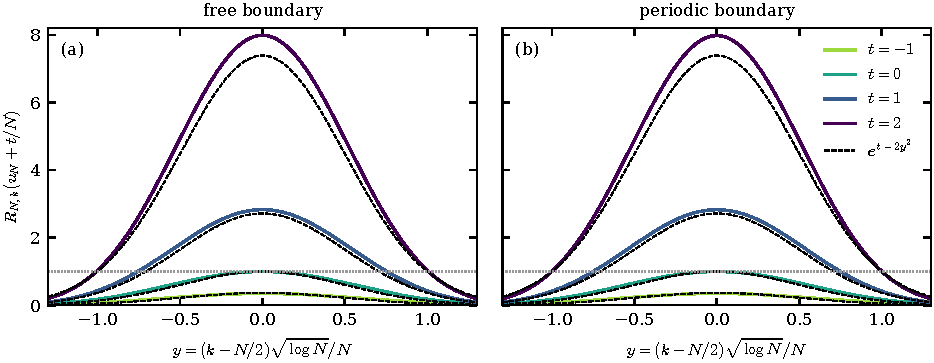
\includegraphics{figures/window}
\caption{The exact ratios $R^X_{N,k}(u_N^X+t/N)$ at $N=10^6$ for free (a) and
periodic (b) boundaries, with the limit $e^{t-2y^2}$ of
Theorem~\ref{thm:critical-window} (dashed). Here $y=(k-N/2)\sqrt{\log N}/N$,
and the bins above the dotted line are above the endpoint height. The
convergence is slow, and at $t=2$ and $y=0$ the relative error is still $0.08$.}
\label{fig:window}
\end{figure}


\section{Verification and scope}\label{sec:verify}
We also checked the results by computer, using Python with only the
standard library. We compared the exact law with a dynamic program and with
a list of every word, and the periodic run polynomial with a separate count
of cyclic words. We also checked the coefficient identities and the order of
the crossings, and evaluated the Bessel bounds and expansions to high
precision. None of the proofs use these checks. \texttt{SUPPLEMENT.md} lists
the scripts and the parts that are proved in Lean, and the output is in
\texttt{data/}. The case of more than two directions is in a separate paper.

\paragraph{Data and code availability.}
The manuscript source, verification scripts, and recorded results are
in the Problem 131 folder of
\url{https://github.com/apemm/Kagey-Problems}.

\begin{thebibliography}{99}\small\setlength{\baselineskip}{11pt}\setlength{\itemsep}{0pt}\setlength{\parsep}{0pt}

\bibitem{kagey131}
P.~Kagey, \emph{Problem 131}, Open Problem Collection,
\url{https://peterkagey.com/problems/131/} (accessed September 2026).

\bibitem{oeisA035002}
E.~Friedman, Sequence A035002, in: OEIS Foundation Inc., \emph{The On-Line Encyclopedia of Integer
Sequences}, \url{https://oeis.org/A035002}.

\bibitem{oeisA348595}
R.~J.~Mathar, Sequence A348595, in: OEIS (2022), \url{https://oeis.org/A348595}.

\bibitem{mathar2022}
R.~J.~Mathar, \emph{Walks of up and right steps in the square lattice with blocked squares}
(January 2022), \url{https://oeis.org/A348595/a348595.pdf}.

\bibitem{goldstein1951}
S.~Goldstein, \emph{On diffusion by discontinuous movements, and on the telegraph equation},
Quart.\ J.\ Mech.\ Appl.\ Math.\ \textbf{4} (1951), 129--156.

\bibitem{gillis1955}
J.~Gillis, \emph{Correlated random walk}, Proc.\ Cambridge Philos.\ Soc.\ \textbf{51} (1955),
639--651.

\bibitem{renshaw1981}
E.~Renshaw and R.~Henderson, \emph{The correlated random walk}, J.\ Appl.\ Probab.\ \textbf{18}
(1981), 403--414.
\url{https://www.jstor.org/stable/3213286}.

\bibitem{waldwolfowitz1940}
A.~Wald and J.~Wolfowitz, \emph{On a test whether two samples are from the same population},
Ann.\ Math.\ Statist.\ \textbf{11} (1940), 147--162.

\bibitem{billingsley1995}
P.~Billingsley, \emph{Probability and Measure}, 3rd ed., Wiley, New York, 1995.

\bibitem{dekkingkong2011}
F.~M.~Dekking and D.~Kong, \emph{Multimodality of the Markov binomial distribution},
J.~Appl.~Probab.\ \textbf{48} (2011), 938--953.
\url{https://arxiv.org/abs/1102.3613}.

\bibitem{herrmann2010}
S.~Herrmann and P.~Vallois, \emph{From persistent random walk to the telegraph noise},
Stochastics and Dynamics \textbf{10} (2010), 161--196.
\url{https://arxiv.org/abs/0810.0650}.

\bibitem{antal2004}
T.~Antal, M.~Droz and Z.~R\'acz, \emph{Probability distribution of magnetization in the
one-dimensional Ising model: effects of boundary conditions},
J.~Phys.~A: Math.~Gen.~\textbf{37} (2004), 1465--1478.
\url{https://arxiv.org/abs/cond-mat/0308442}.

\bibitem{dantchev2022}
D.~Dantchev and J.~Rudnick, \emph{Exact expressions for the partition function of the
one-dimensional Ising model in the fixed-$M$ ensemble},
Phys.~Rev.~E \textbf{106} (2022), L042103.
\url{https://arxiv.org/abs/2207.01134}.

\bibitem{stepanyan2024}
V.~Stepanyan, A.~F.~Tzortzakakis, D.~Petrosyan and A.~E.~Allahverdyan,
\emph{Thermal transitions in a one-dimensional, finite-size Ising model},
J.~Stat.~Mech. (2024), 033202.
\url{https://doi.org/10.1088/1742-5468/ad2679}.

\bibitem{cekanavicius2001}
V.~\v{C}ekanavi\v{c}ius and M.~Mikalauskas,
\emph{Local theorems for the Markov binomial distribution},
Lithuanian Math.~J.~\textbf{41} (2001), 219--231.
\url{https://doi.org/10.1023/A:1012802428342}.

\bibitem{cekanavicius2001ld}
V.~\v{C}ekanavi\v{c}ius and M.~Mikalauskas,
\emph{Large deviations for the Markov binomial distribution},
Lithuanian Math.~J.~\textbf{41} (2001), 307--318.
\url{https://doi.org/10.1023/A:1013840819221}.

\bibitem{dlmf}
NIST, \emph{Digital Library of Mathematical Functions}, Eqs.~10.25.2 and~10.40.1,
and Sec.~18.15(iv),
\url{https://dlmf.nist.gov/10.25.E2}, \url{https://dlmf.nist.gov/10.40.E1},
\url{https://dlmf.nist.gov/18.15}.

\end{thebibliography}

\end{document}
